\subsection{Клиент-серверная архетектура}

Архитектура программного продукта – совокупность важнейших решений об организации программной среды. 

В процессе проектирования архитектуры, программистом определяются основные компоненты разрабатываемой системы и способы (интерфейсы) взаимосвязи этих компонентов. Благодаря предварительной проектировке архитектуры, можно составить план разработки проекта, тем самым избежать множества ошибок.

Большая часть современных приложений представляет собой пример клиент-серверной архитектуры. Данный тип архитектуры описывает распределенные системы, т.е. системы, состоящие из отдельных модулей клиента, сервера и сети, которая соединяет эти модули. 

Главным преимуществом модели клиент-сервер является то, что код клиента и сервера разделен. Все высоконагруженные вычисления происходят на мощный серверах, а клиентская машина, к которым предъявляются менее серьезные требования, не несет большой нагрузки.

Архитектура клиент-сервер в большинстве случаев содержит три типа независимых модулей:
\begin{enumerate}
	\item[1] Клиентский модуль – приложение, написанное на любом языке программирования, и исполняется на стороне клиента. Клиентом может выступать любое приложение, которое может установить соединение с сервером. В веб приложениях клиентом зачастую выступает браузер. В браузере код выполняется на JavaScript. Разработано огромное количество различных JavaScript-библиотек и фреймворков, которые очень сильно облегчают жизнь разработчикам.
	\item[2] Серверный модуль – сервер, на котором исполняется серверное приложение под управлением некоторого веб-сервиса. От выбора веб-сервера зависит язык программирования, который может быть использован для написания серверного приложение, т.е. веб-сервис должен поддерживать интерпретацию этого языка. В список популярных языков серверных приложений можно включить: С\#, Java, Python. Для этих языков разработаны фреймворки и множество библиотек, польза от которых может быть неоценима.
	\item[3] Сервер базы данных. Здесь работает сервер выбранной базы данных. Выбор базы данных – трудоемкое занятие, требующее учитывать множество различных факторов, один из основных – размер базы данных. MS SQL Server, Oracle, PostgreSQL, DB2 – варианты для тяжелых проектов, т.е. для таких которые требуют хранения большого объема данных. Для проектов, требования к объему базы данных меньше, могут подойти MySQL, MongoDB, Interbase.
\end{enumerate}

Существует два вида архитектуры взаимодействия клиент-сервер: первый получил название двухуровневая архитектура клиент-серверного взаимодействия, второй – многоуровневая архитектура клиент-сервер (иногда его называют трехуровневая архитектура или трехзвенная архитектура, но это частный случай). Двухуровневая клиент-серверная архитектура является самой простейшей реализацией архитектуры клиент-сервер, она состоит из серверного приложения и клиентского модуля.

\subsubsection{Двухуровневая архитектура}

Принцип работы двухуровневой архитектуры взаимодействия клиент-сервер заключается в том, что обработка запроса происходит на одной машине без использования сторонних ресурсов. Двухуровневая архитектура проще, так как все запросы обслуживаются одним сервером, из-за этого она более надежна но предъявляет повышенные требования к производительности сервера.

\begin{figure}[h!]
	\centering
	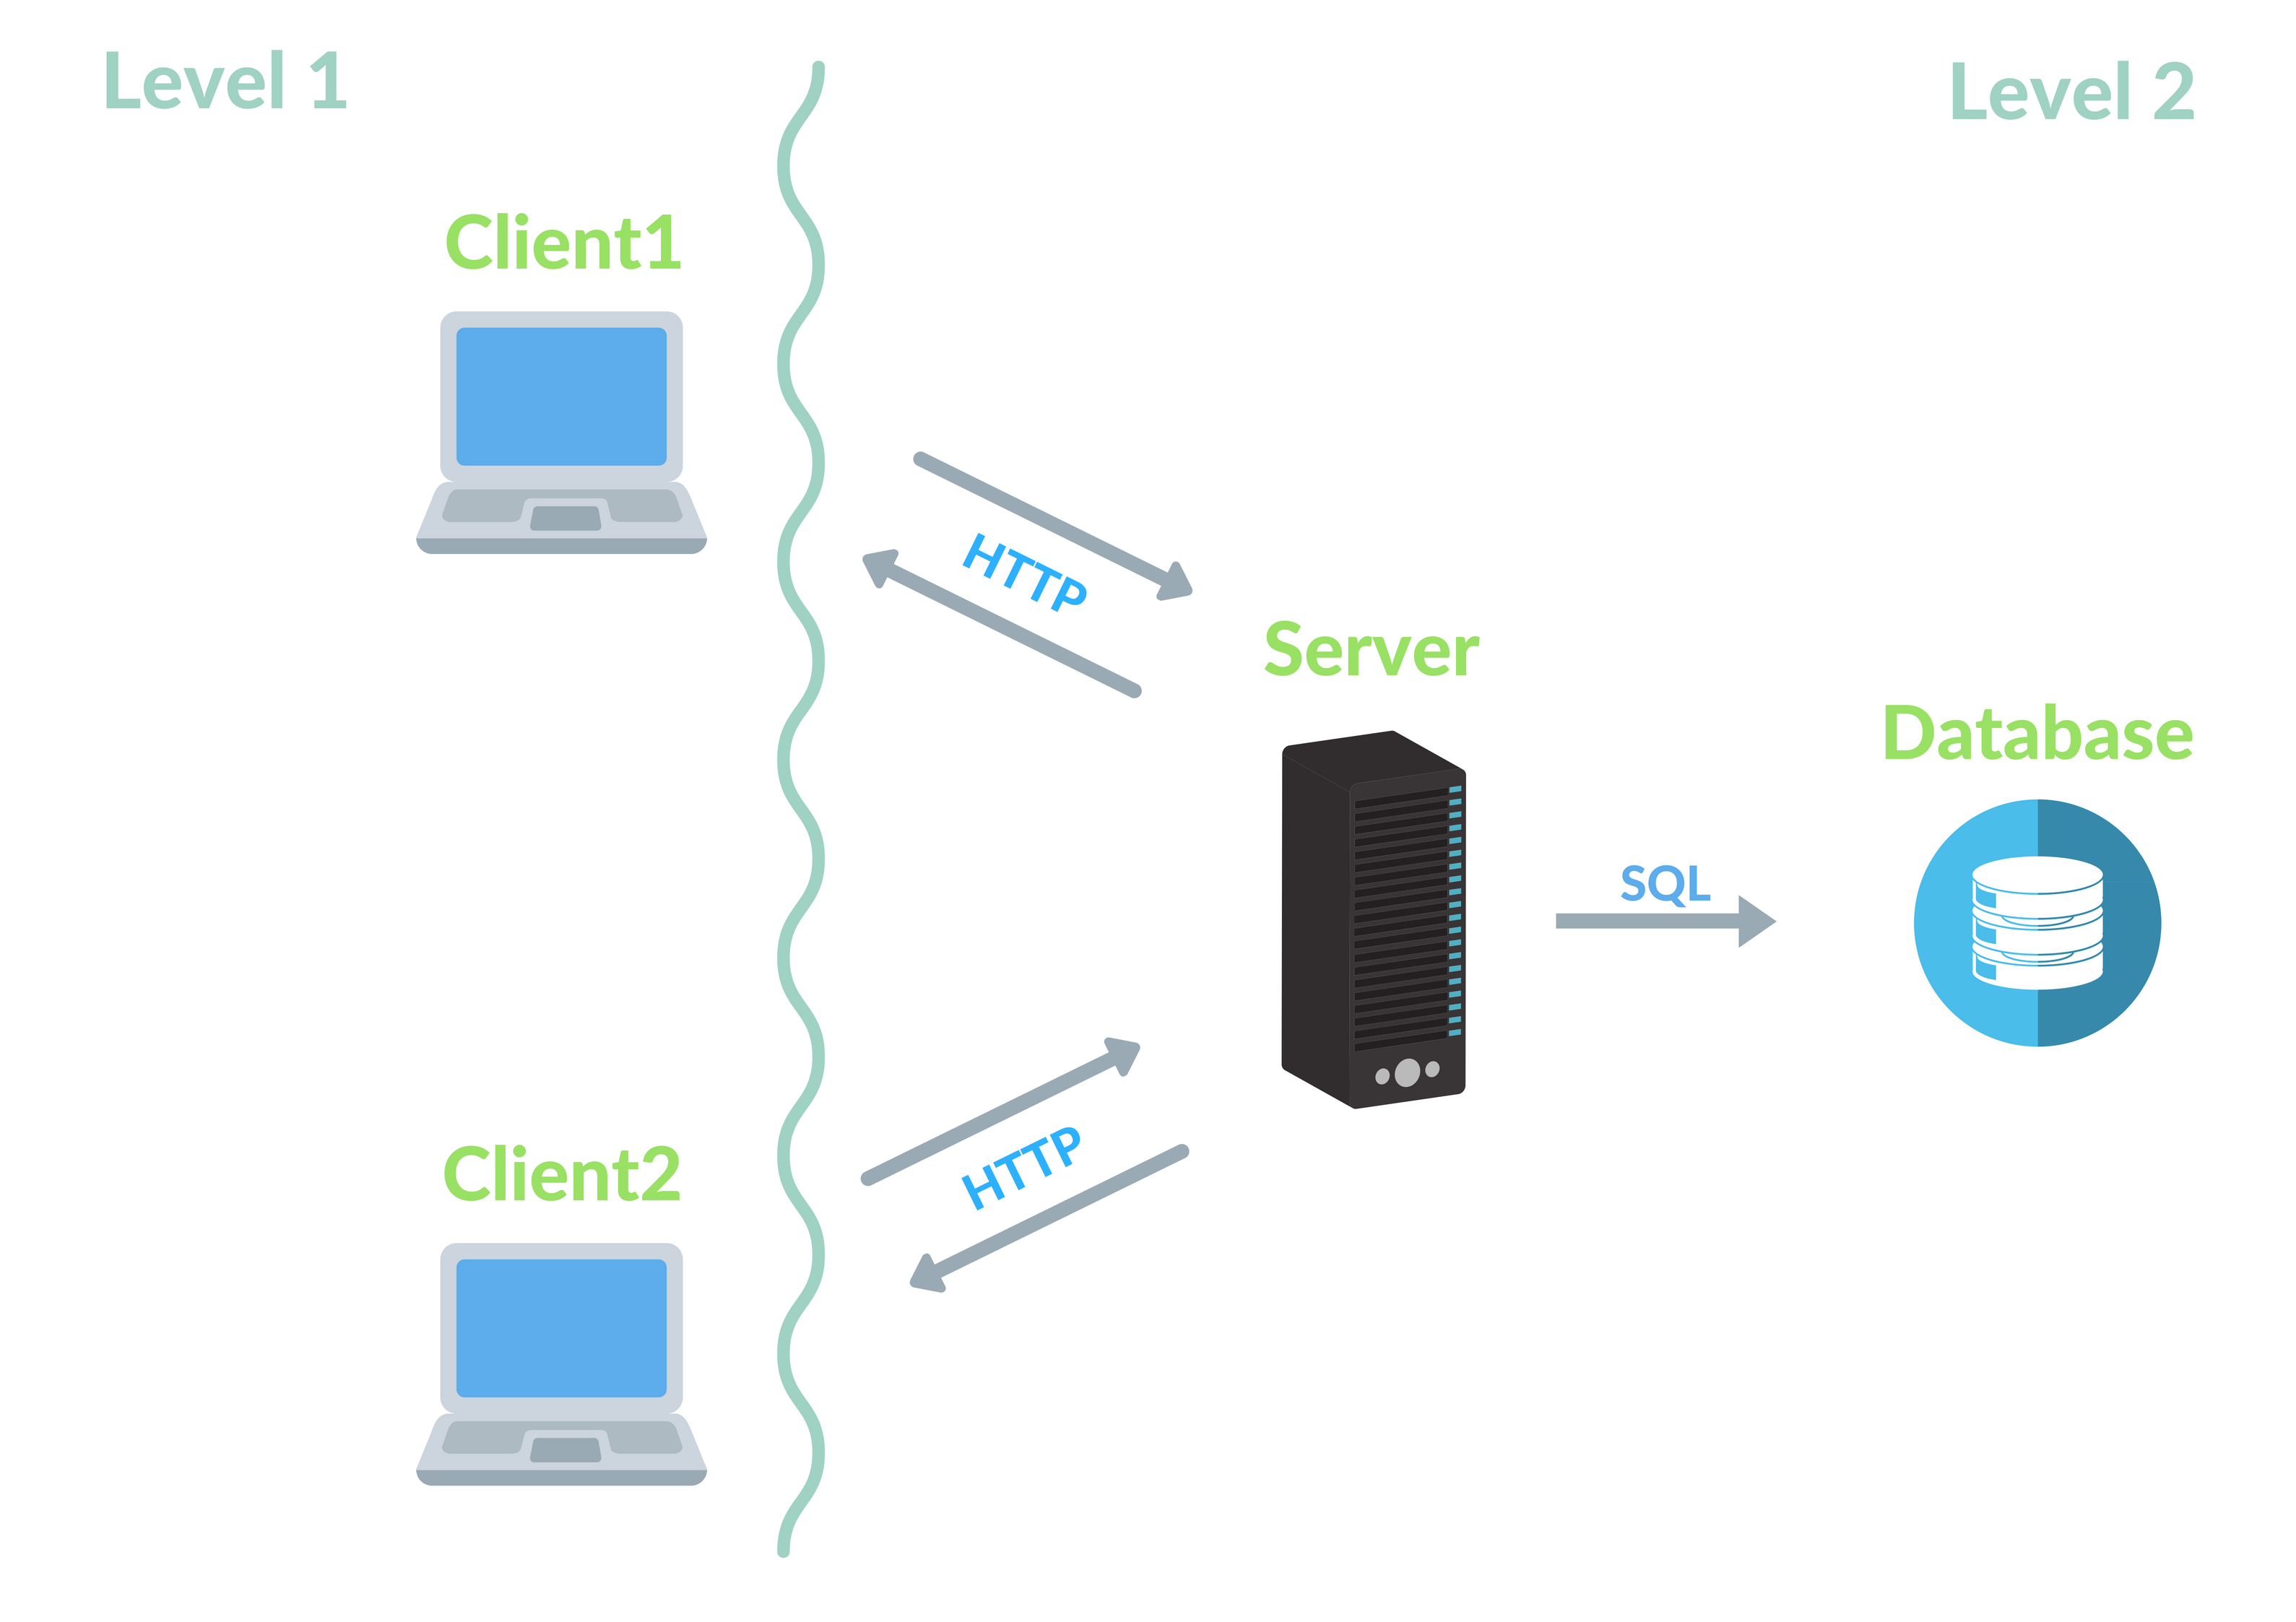
\includegraphics[scale=0.12]{2arch.png}
	\caption{Схема двухуровневой архитектуры}
	\clearpage
\end{figure}

Здесь четко видно, что есть два клиента на первом уровне, который позволяет им сделать запрос, и есть сервер, который обрабатывает запросы клиентов.
\subsubsection{Трехуровневая архитектура}

Если говорить про многоуровневую архитектуру взаимодействия клиент-сервер, то в качестве примера можно привести любую современную СУБД (за исключением библиотеки SQLite, которая в принципе не использует концепцию клиент-сервер). Суть многоуровневой архитектуры заключается в том, что запрос клиента обрабатывается сразу несколькими серверами. Такой подход позволяет значительно снизить нагрузку на сервер из-за того, что происходит распределение операций, но в то же самое время данный подход не такой надежный, как двухуровневая архитектура (рисунок 6.1). Трехзвенная архитектура сложнее, но это достойная цена за пользу, которую может принести распределение функций между серверами второго и третьего уровня.

Трехзвенная архитектура клиент-сервер имеет следующие основные преимущества:
\begin{enumerate}
	\item Высокая степень гибкости и масштабируемости. Может быть расширена путем выделения дополнительных серверов, каждый из которых будет представлять собственные сервисы и пользоваться услугами прочих серверов разного уровня.
	\item Высокая степень безопасности. Защиту можно определить для каждого сервиса или уровня.
	\item Высокая производительность. Задачи распределены между серверами.
\end{enumerate}

Взаимодействие клиента с сервером, при такой архитектуре, происходит путем запросов. Т.е. клиент отправляет запрос на сервер, для совершения некоторого действия, сервер получает запрос, взаимодействует с базой данных, обрабатывает полученные данные из базы и после отправляет обратно к клиенту.

Типичный пример трехуровневой модели клиент-сервер. Если говорить в контексте систем управления базами данных, то первый уровень – это клиент, который позволяет нам писать различные SQL запросы к базе данных. Второй уровень – это движок СУБД, который интерпретирует запросы и реализует взаимодействие между клиентом и файловой системой, а третьим уровнем является хранилище данных.

Учтя всё вышесказанное, можно смоделировать клиент-серверную структуру для нашего приложения. Она будет представлена трехуровневой системой. На первом уровне располагаются веб-клиент СЭД и клиент MRScan. Веб клиент занимается основной обработкой всего функционала документооборота, направляя запросы на сервер(3-й уровень), сервер в свою очередь обращается к серверу базы данных для получения необходимых данных. Клиент MRScan передает серверу отсканированные файлы по технологии WCF. Схема архитектуры проекта представлена на рисунке 6.2.

\begin{figure}[h!]
	\centering
	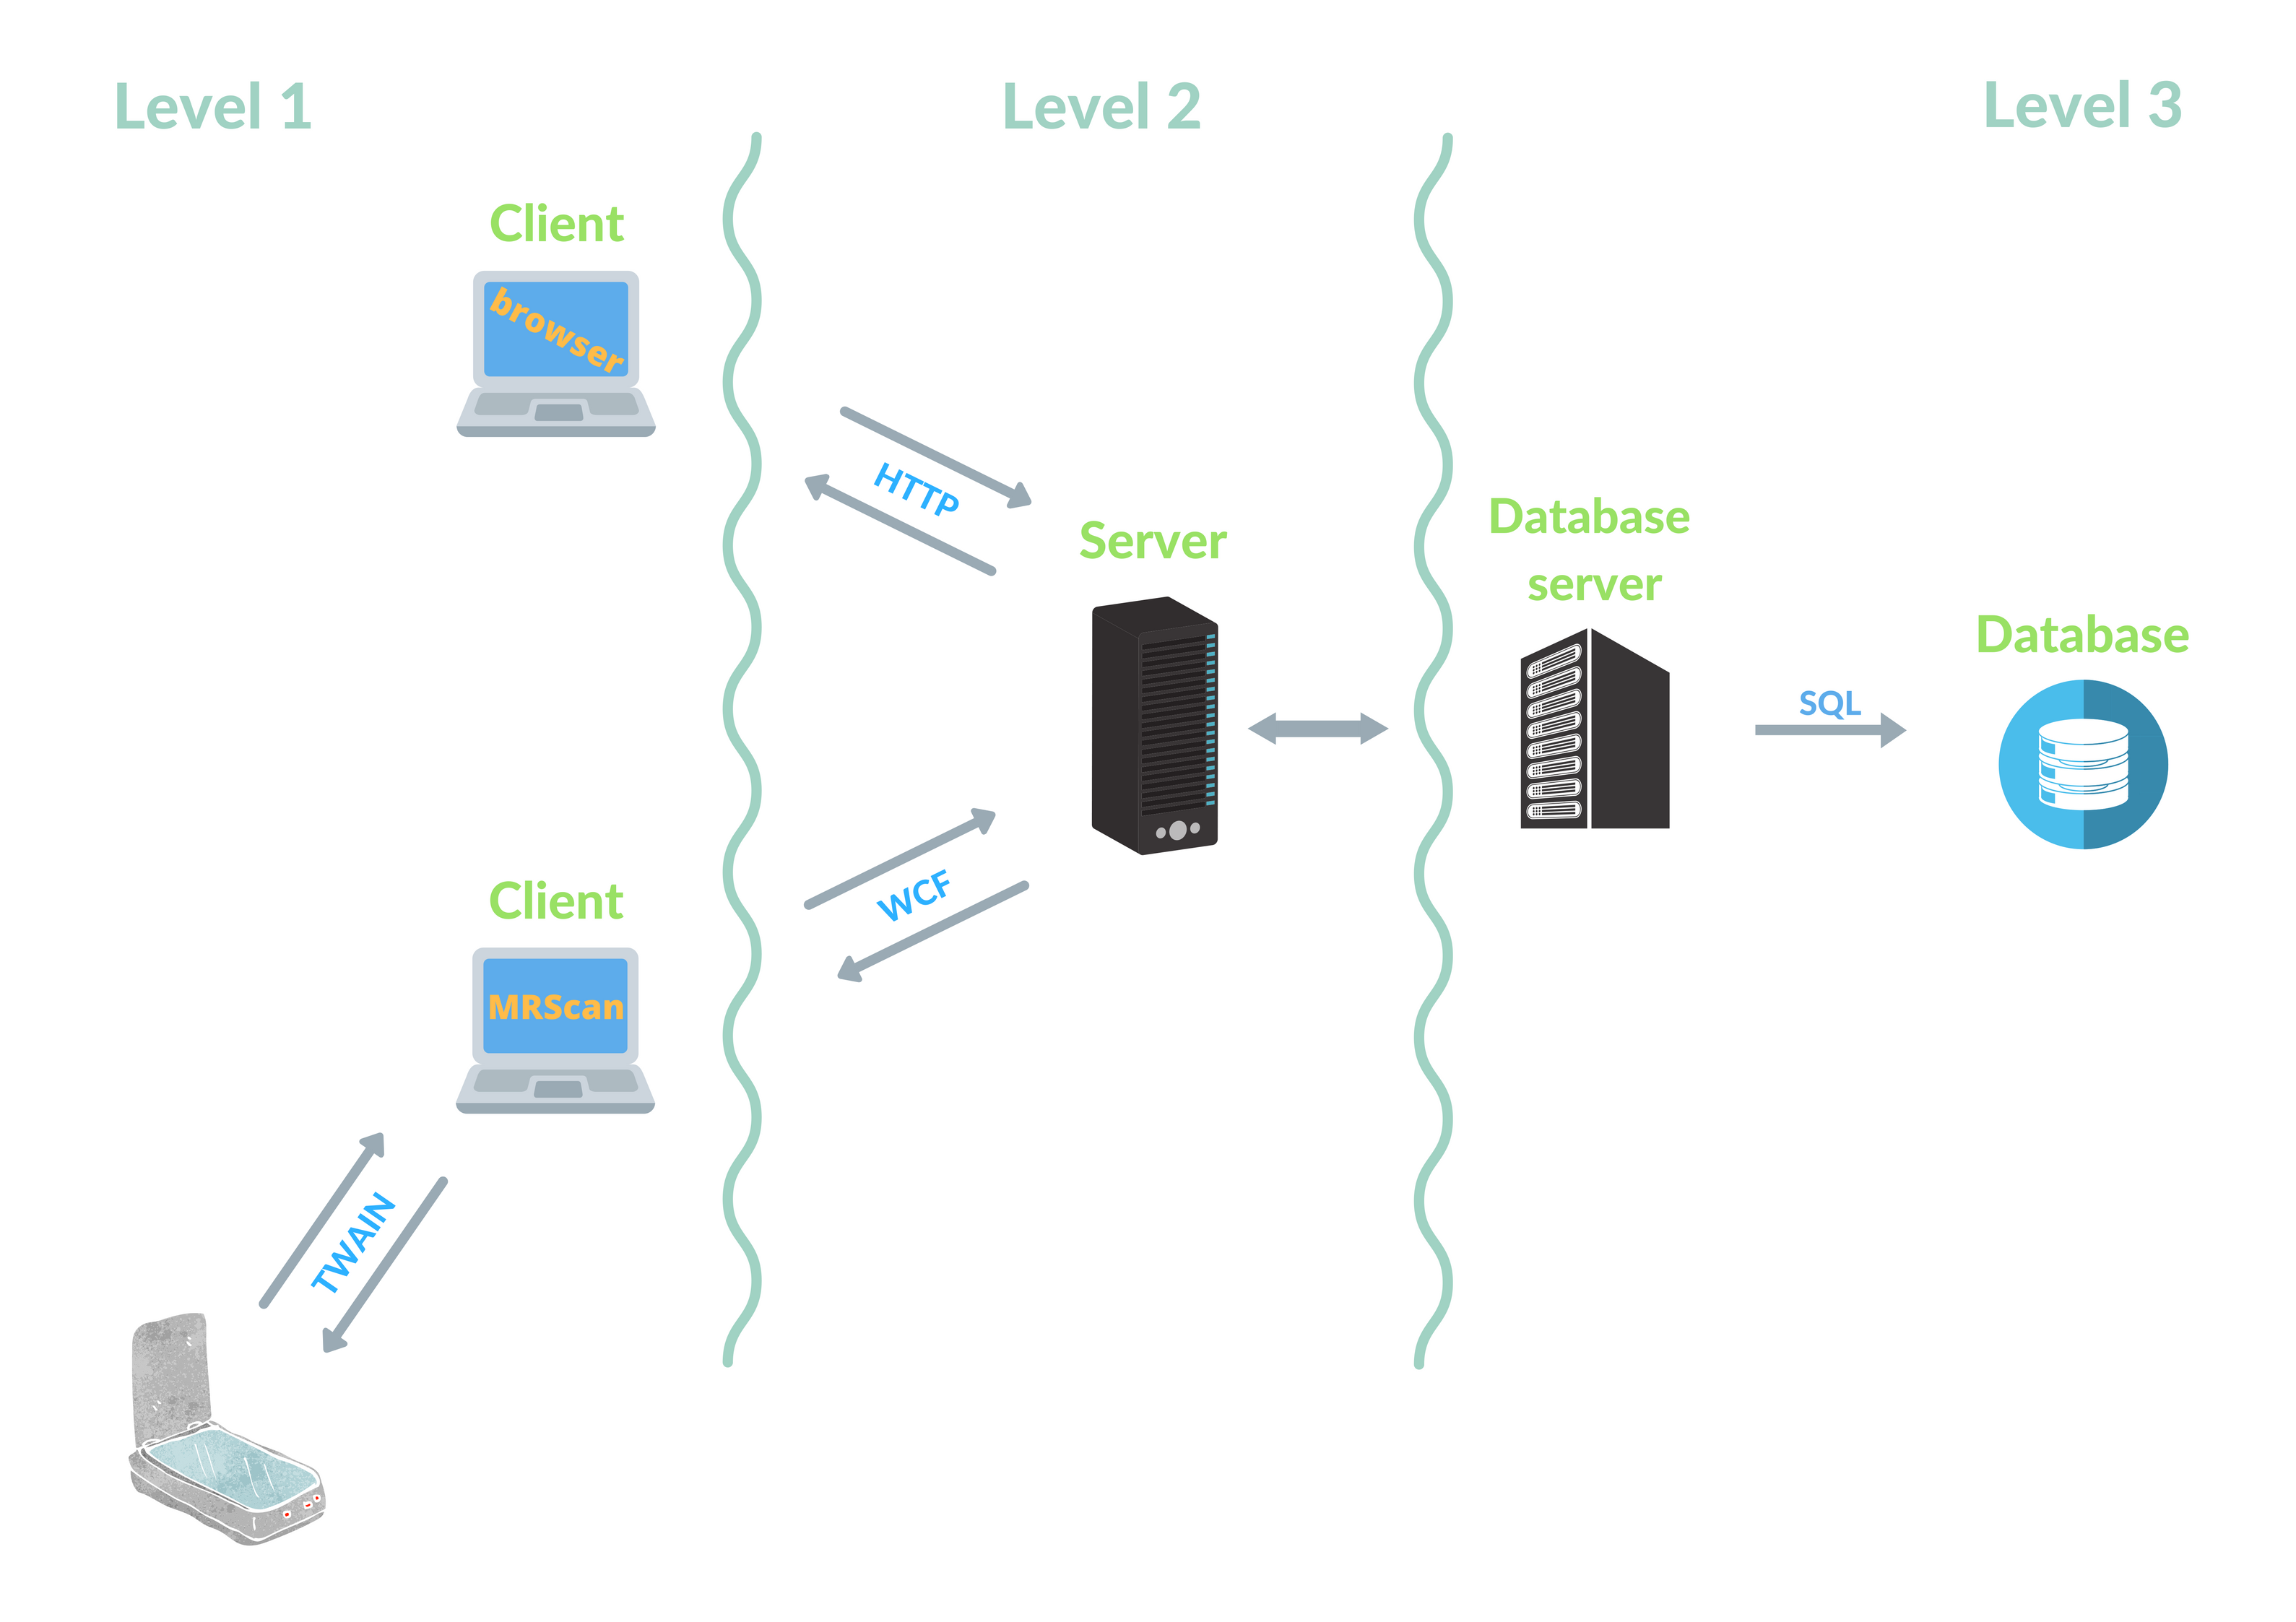
\includegraphics[scale=0.15]{architecture.png}
	\caption{Схема архитектуры проекта}
	\clearpage
\end{figure}